\chapter{METODOLOGIAS E ANÁLISES}
\label{cap:metodologias e analises}

Ao decorrer do processo de pesquisa, foi executado uma revisão da literatura obtida através por chaves duplas {(Natural Language + Model Generation), (Natural Language + Test Model), (Requirement Document + Test Model), (Requirement Document + Information Extraction), (Requirement Document + Model Generation), (Natural Language + State Model), (Natural Language + State Machine), (Natural Language + Automation Test), (Natural Language + Automaton Generation)} onde foi coletado de diversas bases de dados, toda a literatura necessária para a fundamentação teórica do presente projeto bem como uma futura revisão sistemática para publicação.

Paralelamente a tal busca, um conjunto de ferramentas e bibliotecas conhecidas para processamento de línguas naturais (PLN) de código aberto, sob licença GNU/GPL - General Public License foram testadas objetivando o estudo do comportamento de seus algorítimos, taxas de sucesso/fracasso, informações de saída e entrada bem como suas implementações (neste caso avaliando possibilidades de alteração do código para o idioma português brasileiro, uma vez em que tais ferramentas trabalham com idioma Inglês, espanhol, dentre outros.).

\subsection{Stanford CoreNLP – Natural language software}
A primeira ferramenta a ser avaliada perante seu comportamento e sua estrutura estudada na pesquisa do presente projeto foi o parser de Stanford, CoreNLP. Aferiu-se que a ferramenta possui uma alta taxa de sucesso na estimativa das estruturas de um corpus de aproximadamente 98\% de sucesso. Esses altos índices de acerto deve-se ao fato de sua implementação interna atrelado ao uso de algorítimos para parsing como o poderoso parser Charniak, conforme verificou-se em estudos de sua estrutura de core.

\begin{figure}[H]
\centering
\caption{Implementações do software CoreNLP} %legenda
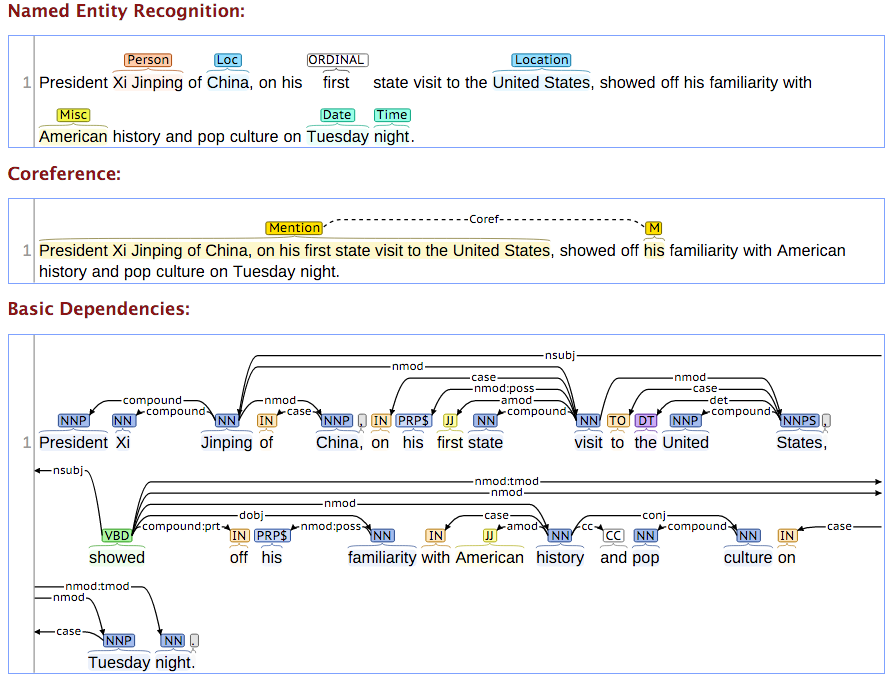
\includegraphics[scale=0.4]{03}\\  % o 0.9 indica 90% do tamanho original
{\small Fonte: Stanford CoreNLP - https://stanfordnlp.github.io} %Fonte da imagem
\label{fig:exemplo} %rotulo para refencia
\end{figure}

Em um primeiro momento, a presente ferramenta foi o principal candidato para a incorporação no sistema proposto no projeto, viável, uma vez em que possui licença GNU/GPL - General Public License e código aberto. Seria necessário desenvolver e adicionar um módulo para o processamento de língua no idioma Português, haja visto que a ferramenta implementa o seguinte conjunto de idiomas: Árabe, Inglês. Espanhol, Alemão, Frances e Chines. Os resultados de tal escolha e modificação serão discutidos posteriormente na seção de de Resultados deste documento.

\subsection{Poli-Libras}
Uma ferramenta de tradução automática de textos escritos em idioma português para sequencia de sinais de Libras (Linguagem Brasileira de Sinais) por meio de interface gráfica e vetores que representam uma personagem humana reproduzindo os sinais traduzidos. O poli-libras conta com diversos módulos, onde demonstra-se viável o reaproveitamento e a incorporação (haja visto que ambos o projeto possui licença GNU/GPL - General Public License) ao projeto apresentado por via do presente documento.

Um módulo encontrado na implementação do Poli-Libras é útil: Módulo de geração da árvore sintática responsável pelo processo de parsing de um determinado corpus redigido em idioma Português brasileiro.

\begin{figure}[H]
\centering
\caption{Projeto arquitetural do software Poli-Libras} %legenda
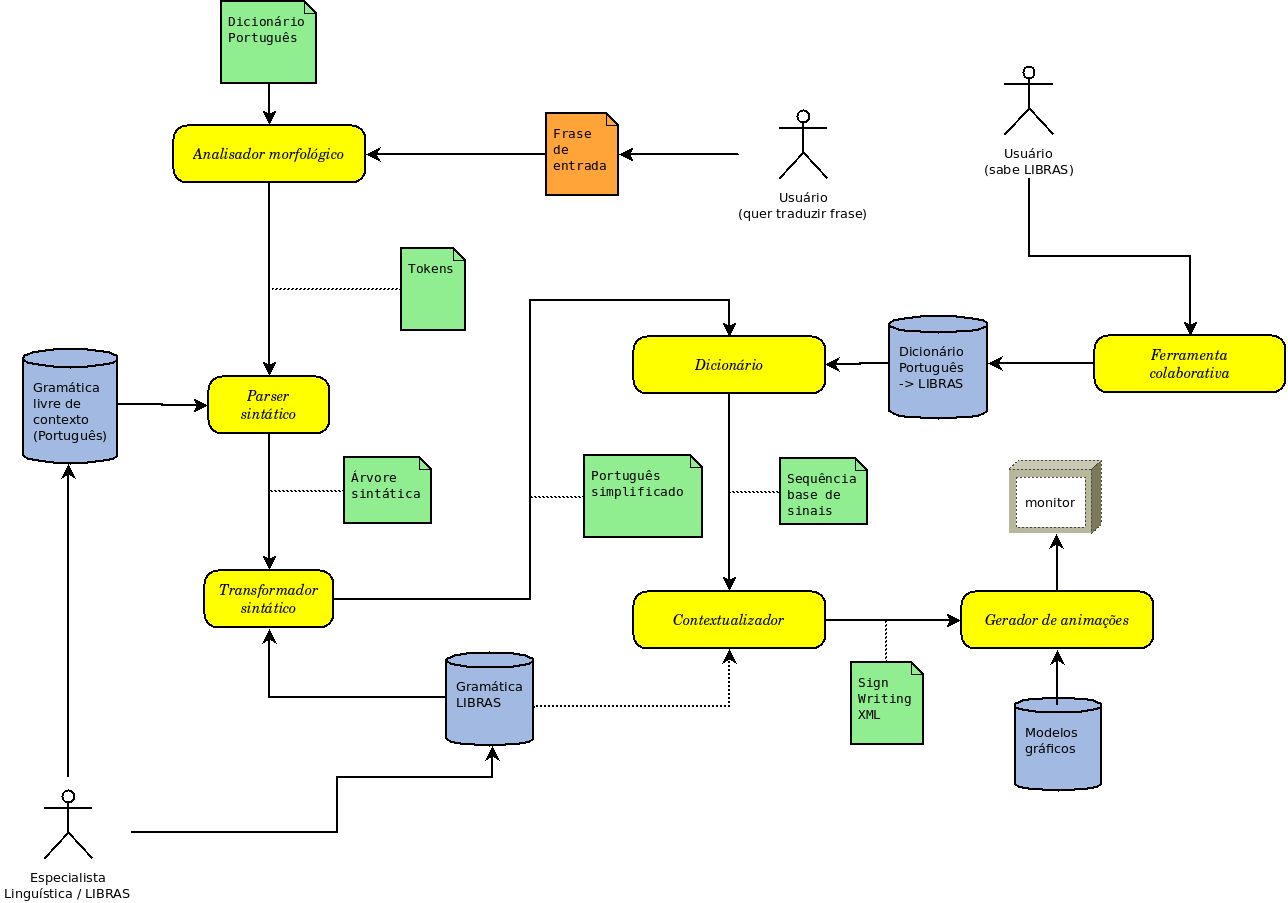
\includegraphics[scale=0.325]{arquitetura}\\  % o 0.9 indica 90% do tamanho original
{\small Fonte: Poli-Libras - http://www.polilibras.com.br/desenvolvimento/tradutor} %Fonte da imagem
\label{fig:exemplo} %rotulo para refencia
\end{figure}

\subsection{NILC's Taggers}
Uma ferramenta tagger utilizada para mapear um corpus textual, classificando todos os termos que o compõem em classes gramaticais, que posteriormente, poderão ser analisados pelo módulo de parsing do projeto para se obter a árvore sintática e assim, tornar possível a extração de informações com base em construções gramaticais conhecidas.

Essa ferramenta trabalha com um padrão internacional e pré estabelecido para definições das tags (tagset), denominado MXPOST, onde a implicação deste fato, será posteriormente abordado no presente documento.


\subsection{CoGrOO - Corretor Gramatical}
A descoberta da ferramenta CoGrOO será abordada posteriormente no presente documento. CoGrOO é uma ferramenta desenvolvida para a suíte de ferramentas Libre Office, de licença livre GNU/GPL - General Public License Version 3.0 e open source, responsável pela analise de corpus textuais objetivando a identificação de erros gramaticais segundo o idioma Português brasileiro.

A ferramenta demonstra-se poderosa e capaz de detectar os seguintes erros gramaticais: colocação pronominal; concordância nominal; concordância entre sujeito e verbo; concordância verbal; uso de crase; regência; nominal; regência verbal.

\subsection{Análise}
Todas as ferramentas supracitadas foram analisadas quanto ao nível de input e output, objetivando se as saídas produzidas cobrem as necessidades do vingante projeto como por exemplo a construção da árvore sintática, a classificação das estruturas gramaticais, um corpus pré processado por um tagger, dentre outros aspectos.
Ao decorrer da presente fase de desenvolvimento da pesquisa, estudou-se toda a estrutura e arquitetura das ferramentas analisadas, possibilitado pela natureza open source.